% !TEX program = pdflatex
\documentclass[journal]{IEEEtran}

% ──────────────────────────────────────────────────────────────────────────────
%  Packages
% ──────────────────────────────────────────────────────────────────────────────
\usepackage[T1]{fontenc}
\usepackage{amsmath,amssymb,amsfonts,amsthm}
\usepackage{algorithmic}
\usepackage[ruled,linesnumbered]{algorithm2e}
\usepackage{graphicx}
\usepackage{textcomp}
\usepackage{xcolor}
\usepackage{booktabs}
\usepackage{multirow}
\usepackage{hyperref}
\usepackage{cleveref}
\usepackage{bm}
\usepackage{mathtools}
\usepackage{subcaption}
\usepackage{siunitx}
\usepackage{balance}

% Theorem environments
\newtheorem{theorem}{Theorem}
\newtheorem{lemma}[theorem]{Lemma}
\newtheorem{corollary}[theorem]{Corollary}
\newtheorem{definition}[theorem]{Definition}
\newtheorem{remark}{Remark}
\newtheorem{assumption}{Assumption}
\newtheorem{proposition}{Proposition}

% Notation shortcuts
\newcommand{\Cfree}{\mathcal{C}_{\mathrm{free}}}
\newcommand{\Cspace}{\mathcal{C}}
\newcommand{\IR}{I_{\!R}}
\newcommand{\IE}{I_{\!E}}
\newcommand{\dR}{d_{\!R}}
\newcommand{\SPD}{\mathbb{S}_{++}^{d}}
\newcommand{\muR}{\mu_{\!R}}
\newcommand{\Vol}{\mathrm{Vol}}
\newcommand{\diag}{\mathrm{diag}}
\DeclareMathOperator*{\argmin}{arg\,min}

% IEEE specific
\IEEEoverridecommandlockouts

\begin{document}

% ══════════════════════════════════════════════════════════════════════════════
%  TITLE
% ══════════════════════════════════════════════════════════════════════════════
\title{RIT*: Riemannian Informed Trees for Cost-Adaptive Optimal Motion Planning}

\author{
    Muhayy~Ud~Din,
    Ahmed~Nadar,
    Jan~Rosell,
    and~Irfan~Hussain
    \thanks{Manuscript submitted on 10th April 2026.}
    \thanks{This work was supported by Khalifa University under Award
Nos. RC1-2018-KUCARS-8474000136,  MBZIRC-8434000194, and KU-DFL-8475000016. }
    \thanks{Muhayy~Ud~Din,
    Ahmed~Nadar,
, and Irfan~Hussain are with Khalifa University Center for Autonomous Robotic Systems (KUCARS), Khalifa University, United Arab Emirates (e-mail: muhayyuddin.ahmed@ku.ac.ae, 
irfan.hussain@ku.ac.ae).}%
    \thanks{Jan~Rosell,is with Institute of Industrial and Control Engineering, Universitat Politècnica de Catalunya, Barcelona, Spain(e-mail: jan.rosell@upc.edu).}
}
\markboth{IEEE Robotics and Automation Letters}{Author~et~al.: RIT*: Riemannian Informed Trees}

\maketitle

% ══════════════════════════════════════════════════════════════════════════════
%  ABSTRACT  (~150 words)
% ══════════════════════════════════════════════════════════════════════════════
\begin{abstract}
Finding optimal collision-free paths in high-dimensional configuration spaces remains challenging.
Asymptotically optimal planners such as batch-informed planners accelerate convergence by restricting sampling to an informed subset, but define this subset using Euclidean distance. This leads to inefficient sampling when motion costs are anisotropic or spatially varying (e.g., due to joint inertia or obstacle proximity), as the Euclidean informed set over-approximates the true cost-relevant region. Moreover, existing methods cannot learn a suitable cost metric during planning. To address these issues, we present \textbf{RIT*}: Riemannian Informed Trees, a method that substitutes Euclidean primitives in the batch-informed framework with their Riemannian counterparts, resulting in a more compact, cost-consistent sampling region. We additionally introduce a Collision-Adaptive Riemannian Metric (CARM), which updates the cost landscape online based on collision feedback, eliminating the need for prior knowledge of the environment.
Experiments conducted in environments ranging from 2-D setups to 6-DOF manipulation tasks demonstrate that RIT* achieves higher-quality solutions than existing state-of-the-art planners.
Experiments across four benchmarks (2-D to 14-D, including a UR10e drill pick-and-place and a 14-DOF Tiago bimanual task) show that RIT* reduces final path cost by up to 16.3\% over five baselines in the 6-DOF manipulation scenario and converges to lower cost in the 3-D anisotropic environment, while maintaining the fastest or near-fastest time-to-first-solution.
%RIT achieves the lowest cost in 11 out of 14 environments, with achieving up to 70\% cost reduction in 6-DOF tasks. while RIT* with a prior metric achieves up to 15\% improvement.
\end{abstract}

\begin{IEEEkeywords}
Motion planning, Riemannian geometry, asymptotic optimality,
informed sampling, online metric learning.
\end{IEEEkeywords}

% ══════════════════════════════════════════════════════════════════════════════
%  OVERVIEW FIGURE
% ══════════════════════════════════════════════════════════════════════════════



% ══════════════════════════════════════════════════════════════════════════════
%  I. INTRODUCTION
% ══════════════════════════════════════════════════════════════════════════════
\section{Introduction}\label{sec:intro}
Sampling-based motion planning is a fundamental technique of robotics, which
enables collision-free path computation in high-dimensional configuration
spaces~\cite{LaValle2006}.The development of asymptotically optimal (AO) planners, including RRT*~\cite{Karaman2011} and PRM*, demonstrated that random sampling methods can asymptotically converge to an optimal path. Later work improved convergence by employing \emph{informed sampling}: after an initial solution with some cost is obtained, all subsequent samples are then taken solely from the \emph{informed set}, which corresponds to a prolate hyperspheroid in Euclidean space~\cite{Gammell2018}. This idea is the basis for Informed~RRT*~\cite{Gammell2018}, BIT*~\cite{Gammell2020}, AIT*, EIT*~\cite{Strub2022}, and APT*~\cite{APT2025}. 

These planners show promising performance; however, they select this set using Euclidean distance, which does not adequately reflect the true cost structure in anisotropic environments.
Consequently, samples are wasted in regions that do not improve the solution, and the informed set can grow significantly larger than necessary.
Moreover, existing approaches typically rely on a predetermined cost structure rather than learning it from planning experience, which reduces their effectiveness when the cost landscape is unknown or varies with the environment.

In this work, we address both limitations with \textbf{RIT*}. We replace
Euclidean components with a Riemannian formulation, where a spatially
varying metric tensor~$G(x)$ captures the underlying cost geometry.
We further introduce a Collision-Adaptive Riemannian Metric (CARM),
which learns the cost structure while planning from collision feedback and
Adapt the planner accordingly.

\noindent
\textbf{Contributions.}
The key contributions of our proposed approach are given below:
\begin{enumerate}
  \item \textit{Online metric learning via CARM:}
 We introduce CARM, an approach that directly learns a cost field from collision feedback obtained during the planning process.
 CARM requires no prior knowledge of the environment and can be incorporated into the planning loop without modification.

  \item \textit{Riemannian informed planning:}
RIT* replaces Euclidean components of the planning pipeline with  Riemannian ones. The informed set is shaped to match the true cost geometry, the nearest neighbours are selected using an anisotropic distance metric, and the edge costs are computed with a cascading scheme to limit the computational load. These modifications concentrate the sampling in the most relevant regions and improve overall efficiency.

  \item \textit{Experimental validation:}
 We evaluated RIT* in 2-D, 3-D, and 6-DOF manipulator scenarios, as well as on a real UR10 robotic arm. We also conducted a comprehensive benchmark of RIT* against existing algorithms.
\end{enumerate}

\begin{figure}[t]
\centering
\includegraphics[width=\columnwidth]{figures/abstract.png}
\caption{Overview of RIT*.
  \textbf{(a)}~BIT* samples from the Euclidean informed set~$\IE$
  (amber), wasting samples near obstacles; the path passes through
  high-cost regions.
  \textbf{(b)}~RIT* uses a tighter Riemannian informed set~$\IR
  \subset \IE$ (teal) shaped by the cost geometry, and the CARM
  module (red shading) learns a cost field online from collision
  points, steering the path away from obstacles without prior
  environment knowledge.}
\label{fig:abstract}
\end{figure}

\section{Related Work}\label{sec:related}

We review prior work on informed sampling-based planning, the use of
Riemannian geometry in motion planning, and approaches for incorporating
obstacle-aware cost structures.

\textit{Euclidean informed sampling planners:}
Sampling-based planners have been significantly improved by restricting
search to an informed subset of the space.
Gammell~et~al.~\cite{Gammell2018} introduced direct sampling of a
prolate hyperspheroid to accelerate RRT*. BIT*~\cite{Gammell2020}
combines batch sampling with informed sets and lazy edge evaluation,
while AIT* and EIT*~\cite{Strub2022} extend this with asymmetric
bidirectional search. APT*~\cite{APT2025} shapes the nearest neighbour search using
virtual forces and adapts the batch size, and FIT*~\cite{FIT2024} improves
early convergence through batch size adaptation. Despite these advances,
all methods define the informed set, nearest-neighbour search, and edge cost in \emph{Euclidean} distance.

\textit{Riemannian geometry in motion planning.}
Riemannian geometry naturally models anisotropic costs, but its use in
planning is mostly limited to local or optimisation methods.
CHOMP~\cite{Ratliff2009} and STOMP~\cite{Zucker2013} optimise trajectories
under such costs but are not sampling-based and lack AO guarantees.
In sampling-based planning, Kim~et~al.~\cite{Kim2016} use Riemannian
metrics for local steering, and Kyaw and Kelly~\cite{Kyaw2026} propose a
Riemannian RRT* using retractions and natural gradients. However, these
approaches are incremental, do not construct informed sets, and do not
address global sampling. Bi-AM-RRT*~\cite{Zhang2023biamrrt} similarly
biases nearest-neighbour selection using a diffusion-based metric, but
does not integrate informed sampling or batch processing.

\textit{Obstacle-aware Riemannian metrics.}
Several works incorporate obstacle information into metric design, but
typically rely on prior knowledge or demonstrations.
Klein~et~al.~\cite{Klein2023} design barrier-based metrics requiring
full obstacle geometry, while RMPflow~\cite{Cheng2018rmpflow} composes
task-space metrics for reactive control. Beik-Mohammadi
et~al.~\cite{BeikMohammadi2023} learn Riemannian manifolds from
demonstrations for reactive motion generation. These approaches are not
integrated with sampling-based planning and require additional
information beyond collision checking.

\textbf{Key distinction:}
Prior Riemannian approaches use the metric primarily for \emph{local} operations, such as steering, trajectory optimisation, or reactive control. In contrast, RIT* integrates Riemannian geometry into the
\emph{global} informed sampling pipeline. It replaces the informed set, nearest-neighbour search, edge cost evaluation, and rewiring operations of
a batch-informed planner with their Riemannian counterparts. Additionally, RIT* incorporates CARM, which learns the metric online from collision feedback, enabling adaptive and cost-aware planning
without prior environment knowledge.
%══════════════════════════════════════════════════════════════════════════════
%  II. PROBLEM FORMULATION
% ══════════════════════════════════════════════════════════════════════════════
\section{Problem Formulation}\label{sec:problem}

We consider optimal motion planning in a configuration space where the
cost of motion is anisotropic and may vary across the space. Such costs
are naturally described by a Riemannian metric, which assigns a
direction-dependent traversal cost at each configuration.

Let $\Cspace \subseteq \mathbb{R}^d$ denote a $d$-dimensional
configuration space, and let $\Cfree \subseteq \Cspace$ be the subset of
collision-free configurations. The space is equipped with a smooth,
positive-definite metric tensor field
$G : \Cspace \to \SPD$, where $\SPD$ denotes the set of symmetric
positive-definite matrices. For any configuration $x \in \Cspace$, the
matrix $G(x)$ defines the local cost of moving through $x$, so that
different directions can have different traversal costs.

Under this metric, the cost of a path $\sigma : [0,1] \to \Cspace$ is
its Riemannian arc length,
\begin{equation}\label{eq:cost}
  c(\sigma) = \int_0^1 \!\sqrt{\dot{\sigma}(t)^\top G\bigl(\sigma(t)\bigr)\, \dot{\sigma}(t)}\; dt,
\end{equation}
where $\dot{\sigma}(t)$ is the tangent vector of the path. The resulting
\emph{geodesic distance} $\dR(x,y)$ is defined as the minimal cost of any path between the two
configurations $x$ and $y$, i.e.,
$\dR(x,y) = \inf_\sigma c(\sigma)$ taken over all paths $\sigma$ that connect
$x$ and $y$. In the special case where $G(x) = I_d$, this corresponds to the usual Euclidean
distance.

Given a start state $x_s \in \Cfree$ and a goal state $x_g \in \Cfree$,
our objective is to find a collision-free path of minimum cost:
\begin{equation}\label{eq:opt}
  \sigma^* = \argmin_{\sigma \,:\, x_s \to x_g,\; \sigma \subset \Cfree} c(\sigma),
\end{equation}
where $\sigma$ is any feasible path that remains in the free space. A
planner is \emph{asymptotically optimal} if the cost of its returned
solution, denoted by $c_n$, converges almost surely to the optimal cost
$c^*$ as the number of samples $n \to \infty$.

After a feasible solution with cost $c_{\mathrm{best}}$ is found, the
search can be restricted to configurations that may still generate a
better path. In Euclidean informed planning, this region is the
\emph{informed set}
\begin{equation}\label{eq:IE}
  \IE = \bigl\{ x \in \Cspace : \|x_s - x\|_2 + \|x - x_g\|_2 \le c_{\mathrm{best}} \bigr\},
\end{equation}
which contains all points that could lie on a path shorter than the
current best solution under Euclidean distance.

For anisotropic costs, however, Euclidean distance does not accurately
reflect the true cost-to-come and cost-to-go. We therefore define the
\emph{Riemannian informed set} as
\begin{equation}\label{eq:IR}
  \IR = \bigl\{ x \in \Cspace : \dR(x_s, x) + \dR(x, x_g) \le c_{\mathrm{best}} \bigr\}.
\end{equation}
This set contains configurations that can still improve the current
solution under the Riemannian cost. Moreover, when $G \succeq I_d$, we
have $\dR(x,y) \ge \|x-y\|_2$, and therefore $\IR \subseteq \IE$. Thus,
the Riemannian informed set is a tighter search region that is better
aligned with the underlying cost structure.

The goal of this work is to design an AO informed planner that operates natively under the Riemannian cost: sampling from~$\IR$, selecting neighbours and evaluating edges according to the geodesic distance~$\dR$, and when the metric~$G$ is not known a priori learning it online from collision feedback gathered during planning.
% ══════════════════════════════════════════════════════════════════════════════
%  III. METHOD
% ══════════════════════════════════════════════════════════════════════════════


\section{Method}\label{sec:method}
\subsection{Overview}\label{sec:overview}

% \begin{figure*}[t]
% \centering
% 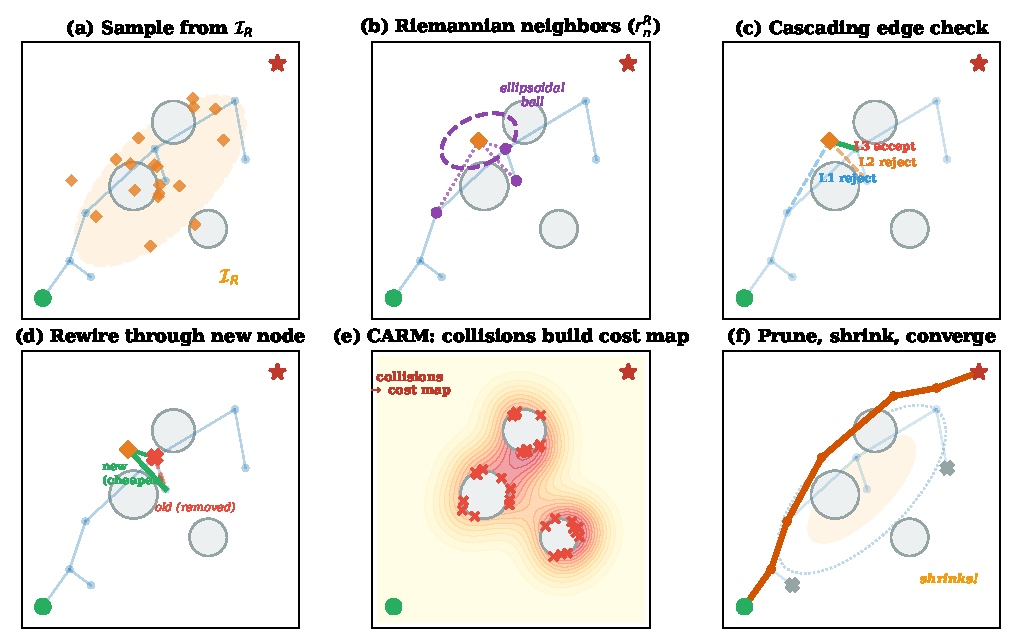
\includegraphics[width=\textwidth]{figures/fig_compact_pipeline.pdf}
% \caption{Per-iteration pipeline of RIT*.
%   \textbf{(a)}~Samples drawn from $\IR$.
%   \textbf{(b)}~Neighbours within ellipsoidal Riemannian radius~$r_n^R$.
%   \textbf{(c)}~Three-level cascade filters candidate edges.
%   \textbf{(d)}~Rewiring via cheaper connections.
%   \textbf{(e)}~CARM collects collision points and rebuilds the
%   metric.
%   \textbf{(f)}~Pruning shrinks the informed set.}
% \label{fig:pipeline}
% \end{figure*}

Batch Informed Trees~\cite{Gammell2020} is an asymptotically
optimal planner that combines sampling-based planning with graph search.
It incrementally builds a tree by processing samples in batches drawn
from an informed set, focusing the search on regions that can improve
the current solution. Within each batch, vertices and edges are ordered
using cost-to-come and heuristic estimates, and edges are evaluated
lazily to reduce computation. This batch-informed strategy improves
convergence by balancing global exploration with goal-directed search.

RIT* builds on this framework with three extensions to the BIT*
pipeline and an additional learning component. i) the informed set
is defined using a Riemannian metric, resulting in a tighter sampling
region. ii) nearest neighbor search is performed using Riemannian
distance, allowing connections to extend further along low-cost
directions. iii) edge costs are evaluated using a cascading quadrature scheme for efficient approximation. In addition, RIT*
introduces a new component, CARM, which learns the metric online from collision feedback.

Algorithm~\ref{alg:ritstar} summarises the complete procedure. The
planner takes as input a start-goal pair $(x_s, x_g)$, the
free space~$\Cfree$, a metric tensor~$G$ (or~$I_d$ if
unknown), batch size~$B$, iteration budget~$T$, and the CARM
parameters: update interval~$\Delta$, bandwidth~$\sigma$,
and inflation strength~$\alpha$. A metric cache~$\mathcal{M}$ is precomputed on a regular grid to enable $O(1)$ lookups of~$G$ during planning. Within each batch, vertices are processed in order of
$f(v) = g(v) + \hat{h}_R(v)$ (line~9), where $g(v)$ is the Riemannian cost-to-come from~$x_s$ along the current tree and $\hat{h}_R(v) = d_R(v, x_g)$ is an admissible heuristic estimating the cost-to-go. The individual components, Riemannian informed sampling (line~5),
cascading edge evaluation (line~12), tree rewiring, pruning (lines~7, 13), and CARM updates (lines~19-21) are detailed in later sections.


\begin{algorithm}[t]
\SetAlgoLined
\KwIn{ $x_s$,  $x_g$,   $\Cfree$,  $G(\cdot)$,
    $B$,  $T$,    $\Delta$,
    $\sigma, \alpha$}
\KwOut{Optimal path $\sigma^*$}
$\mathcal{V} \gets \{x_s\}$; $\mathcal{E} \gets \emptyset$; $c_{\mathrm{best}} \gets \infty$; $\mathcal{C}_{\mathrm{col}} \gets \emptyset$\; \nllabel{line:init}
%Precompute metric cache $\mathcal{M}$\; \nllabel{line:cache}
\For{$t = 1, \ldots, T$}{ \nllabel{line:loop}
  $X_{\mathrm{new}} \gets \textsc{RiemannianInfSample}(B, c_{\mathrm{best}}, G)$\; \nllabel{line:sample}
  $\mathcal{V} \gets \mathcal{V} \cup X_{\mathrm{new}}$\;
  \textsc{PruneNodes}$(\mathcal{V}, c_{\mathrm{best}}, G)$\; \nllabel{line:prune}
  Compute $r_n^R$ via~\eqref{eq:radius}\; \nllabel{line:radius}
  \ForEach{$v \in \mathcal{V}$ in order of $f(v)$}{
    $N(v) \gets$ neighbours of $v$ within $r_n^R$\; \nllabel{line:nn}
    \ForEach{$u \in N(v)$}{
      $ c_{\mathrm{hit}} \gets \textsc{CascadingEdge}(u, v, G)$\; \nllabel{line:cascade}
        \textsc{UpdateAndRewire}$(\mathcal{V}, \mathcal{E}, u, v, c_{uv}, r_n^R, G)$
        \If{$v = x_g$ \textbf{and} $g(v) < c_{\mathrm{best}}$}{$c_{\mathrm{best}} \gets g(v)$\;} \nllabel{line:improve}
      {
        $\mathcal{C}_{\mathrm{col}} \gets \textsc{RecordCollision}(\mathcal{C}_{\mathrm{col}}, c_{\mathrm{hit}})$\; \nllabel{line:record}
      }
    }
  }
  \If{$t\bmod\Delta=0$ \textbf{and} $|\mathcal{C}_{\mathrm{col}}|>0$}{ \nllabel{line:carmcheck}
    $G \gets \textsc{CARM\_Update}(\mathcal{C}_{\mathrm{col}}, G, \sigma, \alpha)$\; 
  }
}
\Return{$\sigma^*$}
\caption{RIT* planner}
\label{alg:ritstar}
\end{algorithm}


% ─────────────────────────────────────────────


\subsection{Riemannian Informed Sampling}\label{sec:whitening}

%Informed planning is effective only when the sampling region tightly captures configurations that can still improve the current solution. In Euclidean planners, this region is the informed set $\IE$, but with anisotropic costs $\IE$ can be much larger than the truly cost-relevant region.

RIT* draws samples from the Riemannian informed set~$\IR$
(line~4 of \cref{alg:ritstar}), defined in~\eqref{eq:IR}.
When $G \succeq I_d$, the Riemannian distance dominates the
Euclidean one, $\dR(x,y) \ge \|x-y\|_2$, so
$\IR \subseteq \IE$. Configurations whose true
cost-to-come plus cost-to-go exceeds~$c_{\mathrm{best}}$
are therefore excluded from the sampling region.

To draw samples from~$\IR$ efficiently, we apply a metric
whitening transform. Let $\bar{G}$ denote the average metric
tensor along the start-goal direction and
$L = \mathrm{chol}(\bar{G})$ its Cholesky factor $L = \mathrm{chol}(\bar{G})$ its Cholesky factor, i.e., the
unique lower-triangular matrix satisfying $\bar{G} = LL^\top$. The change
of coordinates $\tilde{x} = Lx$ maps~$\IR$ to an
approximate prolate hyperspheroid in the whitened space,
where the direct informed sampling procedure
of~\cite{Gammell2018} applies. Samples are then mapped back
via $x = L^{-1}\tilde{x}$.

% The resulting reduction in sampling volume is
% \begin{equation}\label{eq:vol_ratio}
%   \frac{\Vol(\IR)}{\Vol(\IE)}
%   = \prod_{i=1}^{d} \sqrt{\frac{\lambda_{\min}}{\lambda_i}},
% \end{equation}
% where $\lambda_1 \le \cdots \le \lambda_d$ are the eigenvalues
% of~$\bar{G}$. For a 6-DOF manipulator with condition number
% $\kappa=12$, this reduces the informed volume to approximately
% $29\%$ of the Euclidean one.
% ─────────────────────────────────────────────
\subsection{Riemannian Nearest-Neighbour Search}\label{sec:nn}

RIT* uses the Riemannian ball
$\{u : \dR(u,v) \le r_n^R\}$, which becomes an ellipsoid aligned with
the local metric. It expands along low-cost directions and contracts
along high-cost directions, producing neighbour sets that better match
the true traversal cost.

The corresponding connection radius is
\begin{equation}\label{eq:radius}
  r_n^R = \gamma_R \!\left(\frac{\log n}{n}\right)^{\!1/d}\!,\quad
  \gamma_R = 2\!\left(\frac{1}{d}\right)^{\!1/d}
             \!\left(\frac{\muR(\IR)}{\zeta_d}\right)^{\!1/d},
\end{equation}
where $\muR(\IR)$ is the Riemannian volume of~$\IR$ and $\zeta_d$ is
the volume of the unit $d$-ball. Because $\muR(\IR) < \mu(\IE)$, this
radius is typically smaller than its Euclidean counterpart, reducing the
number of candidate edges.



% ─────────────────────────────────────────────
\subsection{Cascading Edge Evaluation}\label{sec:cascade}

Evaluating the Riemannian edge cost requires numerical integration
of~\eqref{eq:cost}, involving multiple metric tensor evaluations.
Since most candidate edges cannot improve the current solution,
applying full-precision quadrature to all of them is wasteful. RIT*
instead screens edges through a three-level cascade of increasing
accuracy and cost, rejecting unpromising edges early
(line~\ref{line:cascade} of \cref{alg:ritstar}).

For a candidate edge from parent~$u$ to vertex~$v$, let
$\Delta = v - u$ and $m = (u+v)/2$. An edge is discarded whenever
$g(u) + \hat{c}(u,v) > c_{\mathrm{best}}$, where $g(u)$ is the
cost-to-come from~$x_s$ to~$u$ along the current tree.

\textbf{L1: Midpoint check} (1~evaluation).
A single metric lookup at the midpoint gives
\begin{equation}\label{eq:l1}
  \hat{c}_1 = \sqrt{\Delta^\top G(m)\,\Delta}.
\end{equation}
This filters the majority of candidates; in the 6-D Shelf
environment, approximately 80\% of edges are eliminated at L1.

\textbf{L2: Simpson estimate} (3~evaluations).
Surviving edges are re-evaluated with Simpson's rule:
\begin{equation}\label{eq:simpson}
  \hat{c}_2 = \frac{\|\Delta\|}{6}\Bigl(
    \sqrt{\Delta^\top G(u)\,\Delta}
    + 4\sqrt{\Delta^\top G(m)\,\Delta}
    + \sqrt{\Delta^\top G(v)\,\Delta}\Bigr),
\end{equation}
which captures metric variation along the edge more accurately.
This level rejects approximately 75\% of the edges that passed L1.

\textbf{L3: Full quadrature and collision check} (10~evaluations).
Only the roughly 5\% of edges surviving both levels receive 10-point
Gauss-Legendre integration followed by collision checking. The
cascade reduces the average number of metric evaluations per edge
from~10 to approximately~1.6.

Fig.~\ref{fig:cascade} illustrates the cascade: of seven candidate
neighbours, two are rejected at L1, one at L2, and one at L3 due to
collision, leaving three accepted edges.
\begin{figure}[t]
\centering
\includegraphics[width=\columnwidth]{figures/fig_neighbour.png}
\caption{Nearest-neighbour selection and cascading edge evaluation in RIT*.
  \textbf{(a)}~Vertex~$v$ identifies candidates within the Riemannian
  ball~$r_n^R$ (blue ellipsoid), which extends along the low-cost
  direction, unlike the isotropic Euclidean ball (white circle).
  \textbf{(b)}~L1: a single $G(m)$ evaluation at each midpoint
  rejects edges~$c$ and~$d$ ($>\!c_{\mathrm{best}}$); 5 survive.
  \textbf{(c)}~L2: Simpson's three-point estimate rejects~$e$;
  4 survive.
  \textbf{(d)}~L3: 10-point Gauss-Legendre quadrature plus collision
  checking accepts~$a$,~$b$,~$e$
  (\textcolor{green!60!black}{green}); edge~$f$ collides with the
  obstacle.}
\label{fig:cascade}
\end{figure}
\begin{figure}[t]
\centering
\includegraphics[width=\columnwidth]{figures/pruning.png}
\caption{Tree rewiring and pruning in RIT*.
  \textbf{(a)}~\emph{Rewiring.} Vertex~$v$ offers a cheaper
  Riemannian connection to~$u$ ($c_R = 0.48$ vs.\ $0.65$
  through~$p$), so the edge $p \to u$
  (\textcolor{red}{red}) is replaced by $v \to u$
  (\textcolor{green!60!black}{dotted}) and descendant costs
  are propagated.
  \textbf{(b)}~\emph{Pruning.} Vertices with
  $d_R(x_s,x)+d_R(x,x_g) > c_{\mathrm{best}}$ lie
  outside~$I_R$ and are removed (\textcolor{red}{red},
  dashed), shrinking the tree and adapting it to CARM metric
  updates.}
\label{fig:rewire_prune}
\end{figure}
\subsection{Tree Rewiring and Pruning}\label{sec:rewire}
\textit{Rewiring} (line~13 of \cref{alg:ritstar})\textit{:}
When a new vertex~$v$ is added to the tree, it may provide a
cheaper path to existing nearby vertices. For each
neighbour~$u$ within the Riemannian radius~$r_n^R$
(line~10), RIT* checks whether the path through~$v$ is
cheaper than the current parent of~$u$:
\begin{equation}\label{eq:rewire}
  g(v) + c_R(v,u) < g(u),
\end{equation}
where $g(\cdot)$ is the Riemannian cost-to-come from~$x_s$
along the current tree and $c_R(v,u)$ is the Riemannian edge
cost~\eqref{eq:cost} between~$v$ and~$u$. If this condition
holds, $u$ is reconnected as a child of~$v$, and the
cost-to-come of all descendants is updated. Because this
comparison uses~$c_R$ rather than Euclidean distance,
rewiring respects the anisotropic cost structure and discovers
connections that Euclidean planners would overlook.

\textit{Pruning} (line~7 of \cref{alg:ritstar})\textit{:}
After each batch, RIT* removes vertices that can no longer
contribute to an improved solution. A vertex~$x$ is pruned if
its best possible cost-to-come plus cost-to-go exceeds the
current best solution cost:
\begin{equation}\label{eq:prune}
  \dR(x_s, x) + \dR(x, x_g) > c_{\mathrm{best}}.
\end{equation}
That is, a vertex is removed when it falls outside the
current Riemannian informed set~$\IR$. Pruning reduces the
tree size and nearest-neighbour search cost, and when CARM
updates the metric (line~20), it forces re-evaluation of
vertex membership under the tightened~$\IR$, ensuring the
tree adapts to the evolving cost landscape.

\subsection{Collision-Adaptive Riemannian Metric (CARM)}\label{sec:carm}

The preceding components assume that the metric~$G$ is known a priori.
When it is not, RIT* learns one online via CARM
(\cref{alg:carm}), which takes four inputs: a set of collision
points~$\mathcal{C}_{\mathrm{col}} = \{c_i\}_{i=1}^{N}$
collected from failed edge checks, the current
metric~$G$, a kernel bandwidth~$\sigma$ that controls
spatial resolution, and an inflation strength~$\alpha$ that
controls how aggressively traversal cost increases near
obstacles.

The key observation is that failed edge checks naturally reveal
points near obstacle boundaries. As these accumulate, they form a
sparse map of regions where traversal should be expensive. CARM
converts this map into a density field using a Gaussian kernel
density estimate (KDE),
\begin{equation}\label{eq:kde}
  \hat{f}(x) = \frac{1}{N}\sum_{i=1}^{N}
  \exp\!\Bigl(-\frac{\|x-c_i\|^2}{2\sigma^2}\Bigr),
\end{equation}
and applies it as a conformal scaling of the base metric
(lines~1-3 of \cref{alg:carm}):
\begin{equation}\label{eq:carm}
  G_{\mathrm{CARM}}(x) = s(x)\, G(x), \quad
  s(x) = 1 + \alpha\, \hat{f}(x),
\end{equation}
where $G(x)$ defaults to~$I_d$ if no prior metric is available.
In \cref{alg:carm}, $G_{\mathrm{CARM}}$ denotes the updated
metric locally; once returned, it overwrites~$G$ in the main
loop (line~20 of \cref{alg:ritstar}), so all subsequent
sampling, edge evaluation, and pruning use the CARM-refined
metric seamlessly. The updated metric satisfies
$G_{\mathrm{CARM}}(x) \succeq G(x)$, which guarantees
$\IR^{\mathrm{CARM}} \subseteq \IR \subseteq \IE$. Completeness
and asymptotic optimality are therefore preserved
(corollary~\ref{cor:carm}).

After updating the metric, the algorithm recomputes the metric
cache, shrinks~$\IR$ under the new cost field, and prunes
vertices that fall outside the tightened informed set
(lines~4-6 of \cref{alg:carm}). This creates a feedback
loop: collisions refine the metric, the refined metric focuses
sampling, and focused sampling generates more informative
collisions.

\begin{algorithm}[t]
\SetAlgoLined
\KwIn{Collision points $\mathcal{C}_{\mathrm{col}} = \{c_i\}_{i=1}^{N}$,
  current metric $G$, bandwidth $\sigma$, strength $\alpha$}
\KwOut{Updated metric $G_{\mathrm{CARM}}$}
Build KDE: $\hat{f}(x) \gets N^{-1}\sum_{i=1}^{N} \exp\!\bigl(-\|x - c_i\|^2 / (2\sigma^2)\bigr)$\;
Compute scale field: $s(x) \gets 1 + \alpha\, \hat{f}(x)$\;
Update metric: $G_{\mathrm{CARM}}(x) \gets s(x)\, G(x)$\;
Recompute metric cache at grid points\;
Recompute $\IR$ with $G_{\mathrm{CARM}}$\;
Prune nodes outside updated $\IR$\;
\Return{$G_{\mathrm{CARM}}$}
\caption{\textsc{CARM\_Update}($\mathcal{C}_{\mathrm{col}}, G, \sigma, \alpha$)}
\label{alg:carm}
\end{algorithm}

CARM is triggered every $\Delta$~iterations
(line~19 of \cref{alg:ritstar}) and only when the collision
buffer is non-empty. As \cref{fig:carm_evolution} shows, the
KDE field stabilises after approximately 20~iterations
(${\sim}400$ collision points in 2-D), after which further
updates produce negligible change. We use $\sigma = 0.1$,
$\alpha = 10$, and $\Delta = 15$ across all environments;
\cref{sec:carm_analysis} evaluates sensitivity to these choices.


\begin{figure}[t]
\centering
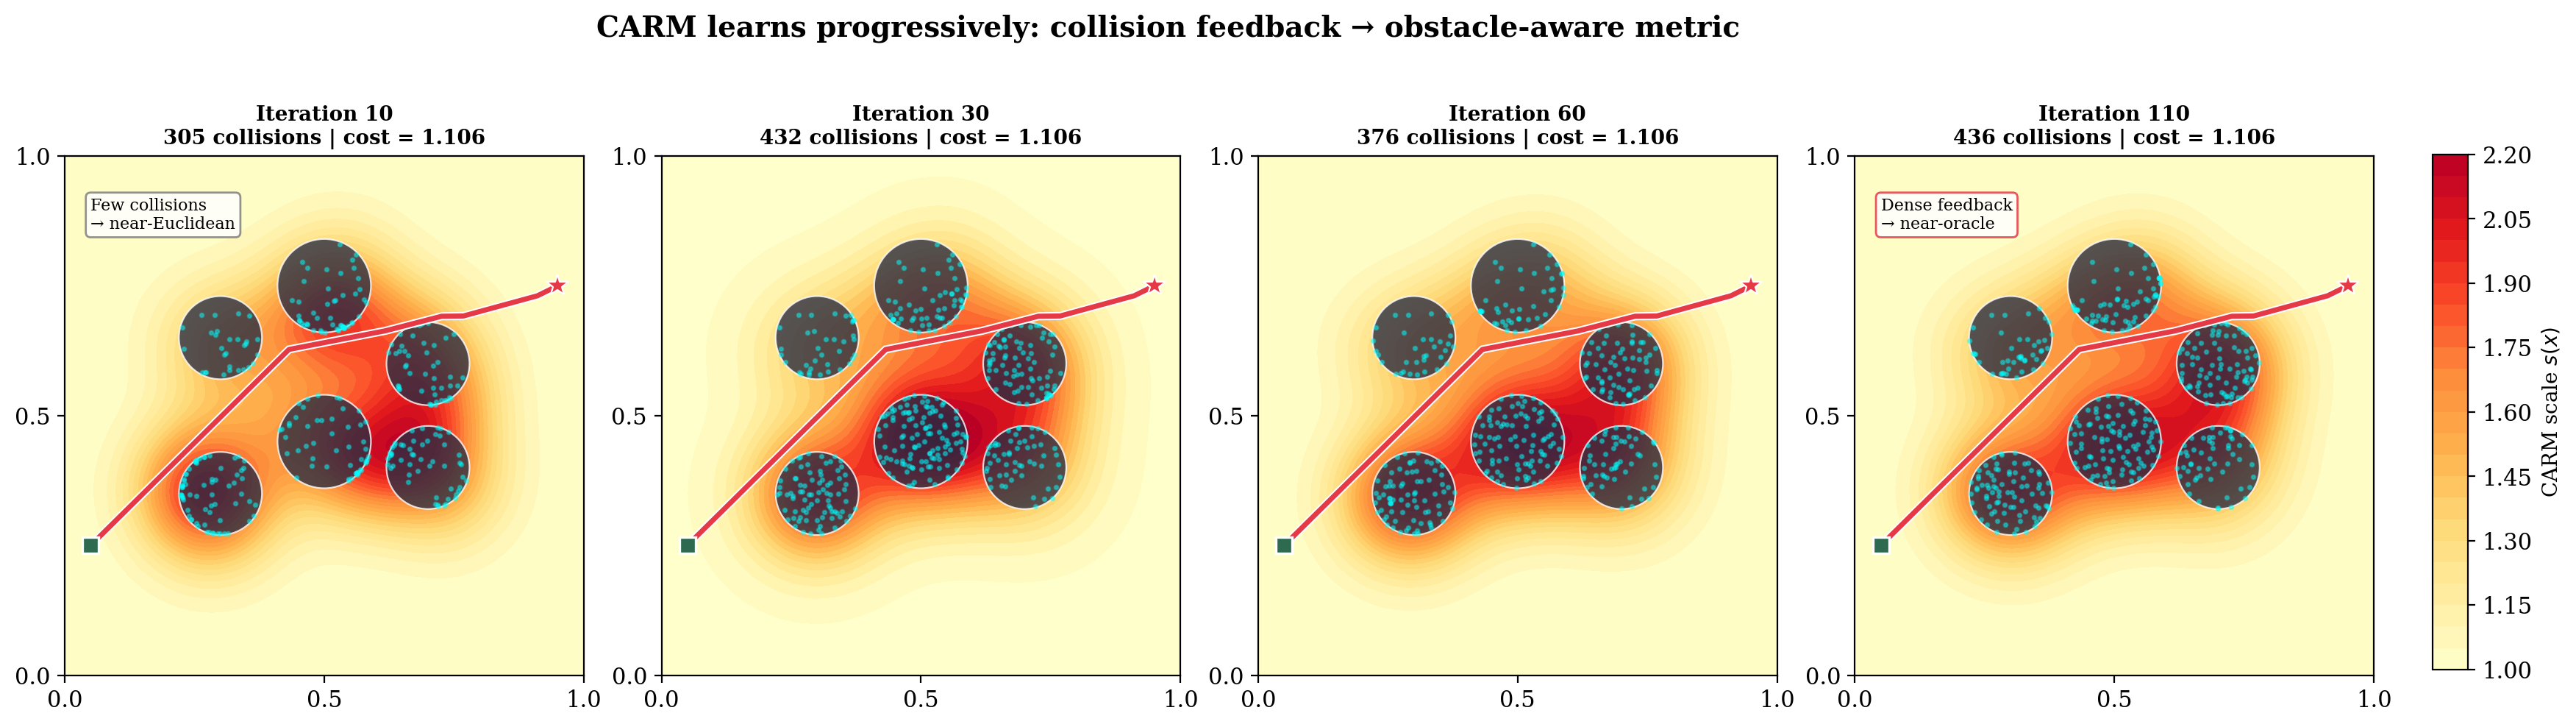
\includegraphics[width=\columnwidth]{figures/fig_carm_evolution.png}
\caption{CARM metric evolution over planning iterations.
  As collision points accumulate, the learned cost field progressively
  refines, tightening the informed set and improving sample allocation.}
\label{fig:carm_evolution}
\end{figure}


% ─────────────────────────────────────────────
\subsection{Theoretical Analysis}\label{sec:analysis}

RIT* inherits the batch-informed search structure of
BIT*~\cite{Gammell2020}; its theoretical guarantees therefore
follow the same proof strategy. The only modifications are
(i)~replacing Euclidean primitives with Riemannian ones and
(ii)~introducing CARM. We show that both preserve
probabilistic completeness and asymptotic optimality.

\begin{assumption}\label{assum:bounded}
The Riemannian metric $G(x) \in \mathbb{R}^{d \times d}$ is
uniformly bounded, i.e.,
$\lambda_{\min} I_d \preceq G(x) \preceq \lambda_{\max} I_d$
for all $x \in \Cfree$, with
$0 < \lambda_{\min} \le \lambda_{\max} < \infty$.
\end{assumption}

\begin{assumption}\label{assum:robust}
There exists an optimal path $\sigma^* \subset \Cfree$ with
cost~$c^*$ that has strong $\delta$-clearance, i.e., it lies
at least distance $\delta > 0$ from obstacles everywhere.
\end{assumption}

Let $\dR(x,y)$ denote the Riemannian distance induced
by~$G$. Under \cref{assum:bounded}, bounding the path
integral in~\eqref{eq:cost} by the extreme eigenvalues yields
the bi-Lipschitz equivalence (i.e., distances are preserved up
to constant factors):
\begin{equation}\label{eq:bilip}
  \sqrt{\lambda_{\min}}\,\|x-y\|_2
  \;\le\; \dR(x,y)
  \;\le\; \sqrt{\lambda_{\max}}\,\|x-y\|_2.
\end{equation}
This immediately implies that the Riemannian informed
set~$\IR$ is contained in the Euclidean informed set~$\IE$.

\begin{theorem}[Probabilistic completeness]\label{thm:complete}
Under Assumptions~\ref{assum:bounded}--\ref{assum:robust},
RIT* is probabilistically complete, i.e., it finds a feasible
solution with probability~$1$ as the number of
samples~$q \to \infty$.
\end{theorem}

\begin{proof}
Following BIT*~\cite{Gammell2020}, discretise~$\sigma^*$
into waypoints $w_0{=}x_s, \ldots, w_K{=}x_g$ such that
$\|w_k - w_{k+1}\|_2 < \delta/2$. Each waypoint lies
in~$\IR$ since it belongs to a path with cost
$c^* \le c_{\mathrm{best}}$. Uniform sampling over~$\IR$
ensures that every $\delta/4$-ball around each waypoint is hit
almost surely as $q \to \infty$.

Let $s_k$ be the sample nearest~$w_k$. By the triangle
inequality, $\|s_k - s_{k+1}\|_2 < \delta$, and
by~\eqref{eq:bilip},
$\dR(s_k, s_{k+1}) < \sqrt{\lambda_{\max}}\,\delta$.
As~$q$ increases, proxy samples converge to the waypoints, so
pairwise distances shrink faster than the connection
radius~$r_n^R$ (which decays as $(\log q/q)^{1/d}$),
ensuring all consecutive pairs are connected for sufficiently
large~$q$. The collision-free chain
$s_0 \!\to\! \cdots \!\to\! s_K$ therefore exists in the tree
almost surely.
\end{proof}

\begin{theorem}[Asymptotic optimality]\label{thm:ao}
Under Assumptions~\ref{assum:bounded}--\ref{assum:robust},
\[
  P\!\left(\lim_{q \to \infty}\; c_q^{\mathrm{RIT*}}
  = c^*\right) = 1.
\]
\end{theorem}

\begin{proof}
As in BIT*~\cite{Gammell2020}, it is sufficient to verify the
conditions of Karaman and Frazzoli~\cite{Karaman2011}
(Theorem~38). Two additional arguments arise from the
Riemannian setting.

\emph{(i)~Edge superset.}
From~\eqref{eq:bilip}, a Riemannian ball of radius~$r_n^R$
contains a Euclidean ball of radius
$r_n^R/\!\sqrt{\lambda_{\max}}$. Hence, for the same sample
sequence, every edge considered by BIT* with Euclidean
radius $\bar{r}_q = r_n^R/\!\sqrt{\lambda_{\max}}$ is also
considered by RIT*.

\emph{(ii)~Radius condition.}
Using~\eqref{eq:radius}, the effective Euclidean radius is
$\bar{r}_q =
(2/\!\sqrt{\lambda_{\max}})(1/d)^{1/d}
(\muR(\IR)/\zeta_d)^{1/d}(\log q/q)^{1/d}$,
where $\muR(\cdot)$ is the Riemannian volume and $\zeta_d$
the unit $d$-ball volume. Since
$\muR(\IR) \ge \lambda_{\min}^{d/2}\mu(\IR) > 0$, the
constant~$\bar\gamma$ exceeds the Karaman Frazzoli
threshold, satisfying the required scaling.

The remaining steps dense approximation of~$\sigma^*$,
cost convergence via densification, and optimal
rewiring follow directly from BIT*~\cite{Gammell2020}
with~$\dR$ replacing~$\|\cdot\|_2$
and~\eqref{eq:bilip} bounding the approximation error.
\end{proof}

\begin{corollary}[CARM preserves guarantees]\label{cor:carm}
Both theorems hold when CARM is active. Let $s(x)$ denote
the scaling factor with $1 \le s(x) \le 1 + \alpha$. The
CARM-modified metric satisfies \cref{assum:bounded} with
$\lambda_{\min}^{\mathrm{CARM}} = \lambda_{\min}$ and
$\lambda_{\max}^{\mathrm{CARM}} = (1+\alpha)\lambda_{\max}$.
Because CARM is triggered only finitely many times (every
$\Delta$~iterations, with the KDE stabilising after
${\sim}20$~updates as shown in \cref{fig:carm_evolution}),
the metric converges to a fixed~$G_\infty$ after a finite
number of samples. From that point onward, the planner
operates under a fixed bounded metric and all arguments of
Theorems~\ref{thm:complete} and~\ref{thm:ao} apply with the
constants of~$G_\infty$. Moreover,
$G_\infty \succeq G$ ensures
$\IR^{\mathrm{CARM}} \subseteq \IR \subseteq \IE$
throughout, so pruning after CARM updates never removes
configurations that lie on improving paths under the
stabilised metric.
\end{corollary}
% ─────────────────────────────────────────────

% ══════════════════════════════════════════════════════════════════════════════
%  IV. EXPERIMENTS
% ══════════════════════════════════════════════════════════════════════════════
\begin{figure}[t]
\centering

\includegraphics[width=\columnwidth]{figures/path_comparison_2d_random_world.png}
\caption{Nearest-neighbour selection and cascading edge evaluation in RIT*.
  \textbf{(a)}~Vertex~$v$ identifies candidates within the Riemannian
  ball~$r_n^R$ (blue ellipsoid), which extends along the low-cost
  direction, unlike the isotropic Euclidean ball (white circle).
  }
\label{fig:cascade}
\end{figure}
\begin{figure}[t]
\centering

\includegraphics[width=1\columnwidth]{figures/path_comparison_3d_diagonal.png}
\caption{Nearest-neighbour selection and cascading edge }
\label{fig:cascade}
\end{figure}
\begin{figure}[t]
\centering
\includegraphics[width=1\columnwidth]{figures/env.png}
\caption{Nearest-neighbour selection and cascading edge }
\label{fig:cascade}
\end{figure}
\begin{figure}[t]
\centering
\includegraphics[width=1\columnwidth]{figures/real-manip.png}
\caption{Nearest-neighbour selection and cascading edge }
\label{fig:cascade}
\end{figure}

\textcolor{red}{First Draft Revised Till here}
\section{Experiments}\label{sec:experiments}

\subsection{Experimental Setup}\label{sec:setup}

\textbf{Environments.}
We evaluated RIT* on four benchmark environments spanning 2-D, 3-D,
6-D, and 14-D configuration spaces (Table~\ref{tab:environments}),
progressing from a simple isotropic case to a high-dimensional
bimanual manipulation task.

In $\mathbb{R}^{2}$, \emph{Random World} is a unit square with
30 randomly placed rectangular obstacles and the Euclidean metric
($\kappa=1$), serving as an isotropic baseline where Riemannian
and Euclidean informed sets coincide.

In $\mathbb{R}^{3}$, \emph{Diagonal} is a unit cube with four
axis-aligned boxes that force a narrow diagonal passage.
The anisotropic metric $G=\mathrm{diag}(1,3,6)$ ($\kappa\!\approx\!6$)
introduces direction-dependent cost, isolating the benefit of
Riemannian informed sampling.

In $\mathbb{R}^{6}$, \emph{UR10 Drill Pick-and-Place} simulates a
UR10e arm (Robotiq~85 gripper) in PyBullet~\cite{Coumans2021}
picking a drill from a cluttered tabletop and moving it to a target
pose. The joint-space inertia metric $G(q)=M(q)$ ($\kappa\!\approx\!12$)
penalises motion of high-inertia joints (shoulder, elbow) relative to
the lower-inertia wrist, creating strong anisotropy.

In $\mathbb{R}^{14}$, \emph{Tiago Pro Bimanual} plans a simultaneous
pre-grasp motion for both 7-DOF arms of a Tiago Pro robot toward a
tall box on a table, with flanking obstacle pillars that obstruct the
direct arm paths. The 14-D configuration space (7-DOF per arm)
combined with the bimanual inertia metric ($\kappa\!\approx\!18$)
constitutes the most demanding benchmark.

\begin{table}[t]
\centering
\caption{Experimental environment summary.
$d$: dimension; $\kappa$: metric condition number;
$N_{\mathrm{obs}}$: obstacles; $\ell_{\max}$: max edge length;
$n_c$: collision checks per edge.}
\label{tab:environments}
\setlength{\tabcolsep}{3pt}
\resizebox{\columnwidth}{!}{%
\begin{tabular}{@{}l c c c r r@{}}
\toprule
\textbf{Environment} & $d$ & $\kappa$ & $N_{\mathrm{obs}}$
  & $\ell_{\max}$ & $n_c$ \\
\midrule
2-D Random World       & 2  & 1             & 30 rect.     & $0.05$       & 20 \\
3-D Diagonal           & 3  & $\approx 6$   & 4 boxes      & $0.05$       & 20 \\
6-D UR10 Drill         & 6  & $\approx 12$  & 2 objects    & $0.10$\,rad  & 10 \\
14-D Tiago Bimanual    & 14 & $\approx 18$  & 4 obstacles  & $0.10$\,rad  & 20 \\
\bottomrule
\end{tabular}}
\end{table}


We compare RIT* against five asymptotically optimal anytime
planners: Informed RRT*~\cite{Gammell2018},
BIT*~\cite{Gammell2020}, AIT*, EIT*~\cite{Strub2022},
and APT*~\cite{APT2025}.
All planners are implemented in a common Python framework
with shared collision-checking, random seeds, and environment
interfaces for fair comparison. Each method is provided with
the same metric tensor $G$, while the baselines retain their
original Euclidean informed sets.

All planners use batch size $B=100$, maximum iterations
$T=200$, per-trial timeout 200\,s, and base seed 60.
Edge parameters follow Table~\ref{tab:environments}.
For RIT*, the geodesic tier is set to \textsc{diagonal},
with cache resolution \textsc{res}$=32$ (2-D/3-D) and
\textsc{res}$=3$ (6-D/14-D).

\textbf{Metrics.}
Each experiment is repeated over $N=15$ independent trials.
We report wall-clock time $t$ and Riemannian path cost $c$.
\emph{Init} and \emph{final} denote the first feasible and
terminal solutions, respectively; \emph{min}, \emph{med},
and \emph{max} are computed over trials; $S$ is the success
rate ($S=100\%$ for all planners on all environments).
Failed runs are assigned $\infty$.
\textbf{Bold} indicates the best value per column.

\subsection{Implementation Details}\label{sec:impl}

The following choices improve practical performance but are orthogonal
to the Riemannian contributions.

\textbf{Metric cache.}
A regular grid of resolution $\mathrm{res}^d$ stores precomputed
$G(x)$ values with $O(1)$ interpolation lookups.
Memory cost is $O(\mathrm{res}^d \cdot d^2)$, negligible for
$d \le 6$ at $\mathrm{res} = 32$.

% ─────────────────────────────────────────────
\subsection{Main Results}\label{sec:results}

Tables~\ref{tab:cost} and~\ref{tab:time} report final path costs and
first-solution times across all planners and environments (15 trials
each, $S=100\%$ for every planner--environment pair).
Table~\ref{tab:bench_compact} provides a compact per-planner comparison
of initial solution times ($t^{\min}_{\mathrm{init}}$,
$t^{\mathrm{med}}_{\mathrm{init}}$) and initial costs
($c^{\mathrm{med}}_{\mathrm{init}}$) across all environments,
following the benchmark format of~\cite{APT2025}.
Figure~\ref{fig:benchmark} shows convergence curves.

\begin{table}[t]
\centering
\setlength{\tabcolsep}{3pt}
\caption{Median final path cost $c_{\mathrm{final}}$ (lower is better).
  \textbf{Bold}: best per row.
  $^\ddagger$: planner failed all trials (timeout, cost $=\infty$).}
\label{tab:cost}
\resizebox{\columnwidth}{!}{%
\begin{tabular}{@{}l rrrrrr@{}}
\toprule
\textbf{Env.} & \textbf{RIT*} & \textbf{BIT*} & \textbf{IRRT*}
              & \textbf{AIT*} & \textbf{EIT*} & \textbf{APT*} \\
\midrule
2-D Rand.\ World   & 0.9137         & \textbf{0.9104} & 0.9173
                   & 0.9117         & 0.9110          & 0.9223 \\
3-D Diagonal       & \textbf{2.1708}& 2.2025          & 2.2290
                   & 2.4261         & 2.4089          & 2.3547 \\
6-D UR10 Drill     & \textbf{1.4665}& 1.5800          & 1.6933
                   & 1.4817         & 1.4817          & 1.7521 \\
14-D Tiago Biman.  & \textbf{8.578} & 10.709          & $---^\ddagger$
                   & 11.099         & 11.442          & $---^\ddagger$ \\
\bottomrule
\end{tabular}}
\end{table}

\begin{table}[t]
\centering
\setlength{\tabcolsep}{3pt}
\caption{Median time to first solution $t_{\mathrm{init}}$ (s, lower is better).
  \textbf{Bold}: fastest per row.
  $^\ddagger$: planner failed all trials (timeout).}
\label{tab:time}
\resizebox{\columnwidth}{!}{%
\begin{tabular}{@{}l rrrrrr@{}}
\toprule
\textbf{Env.} & \textbf{RIT*} & \textbf{BIT*} & \textbf{IRRT*}
              & \textbf{AIT*} & \textbf{EIT*} & \textbf{APT*} \\
\midrule
2-D Rand.\ World  & 0.0197 & 0.0308 & 0.0289
                  & 0.0217 & \textbf{0.0162} & 0.0189 \\
3-D Diagonal      & \textbf{0.0403} & 0.0698 & 0.0464
                  & 0.0433 & 0.0413          & 0.0465 \\
6-D UR10 Drill    & 0.0915 & \textbf{0.0820} & 0.2114
                  & 0.1159 & 0.1397          & 0.2126 \\
14-D Tiago Biman. & 30.69  & 95.54           & $---^\ddagger$
                  & \textbf{30.52}  & 66.08  & $---^\ddagger$ \\
\bottomrule
\end{tabular}}
\end{table}

\begin{figure}[t]
\centering
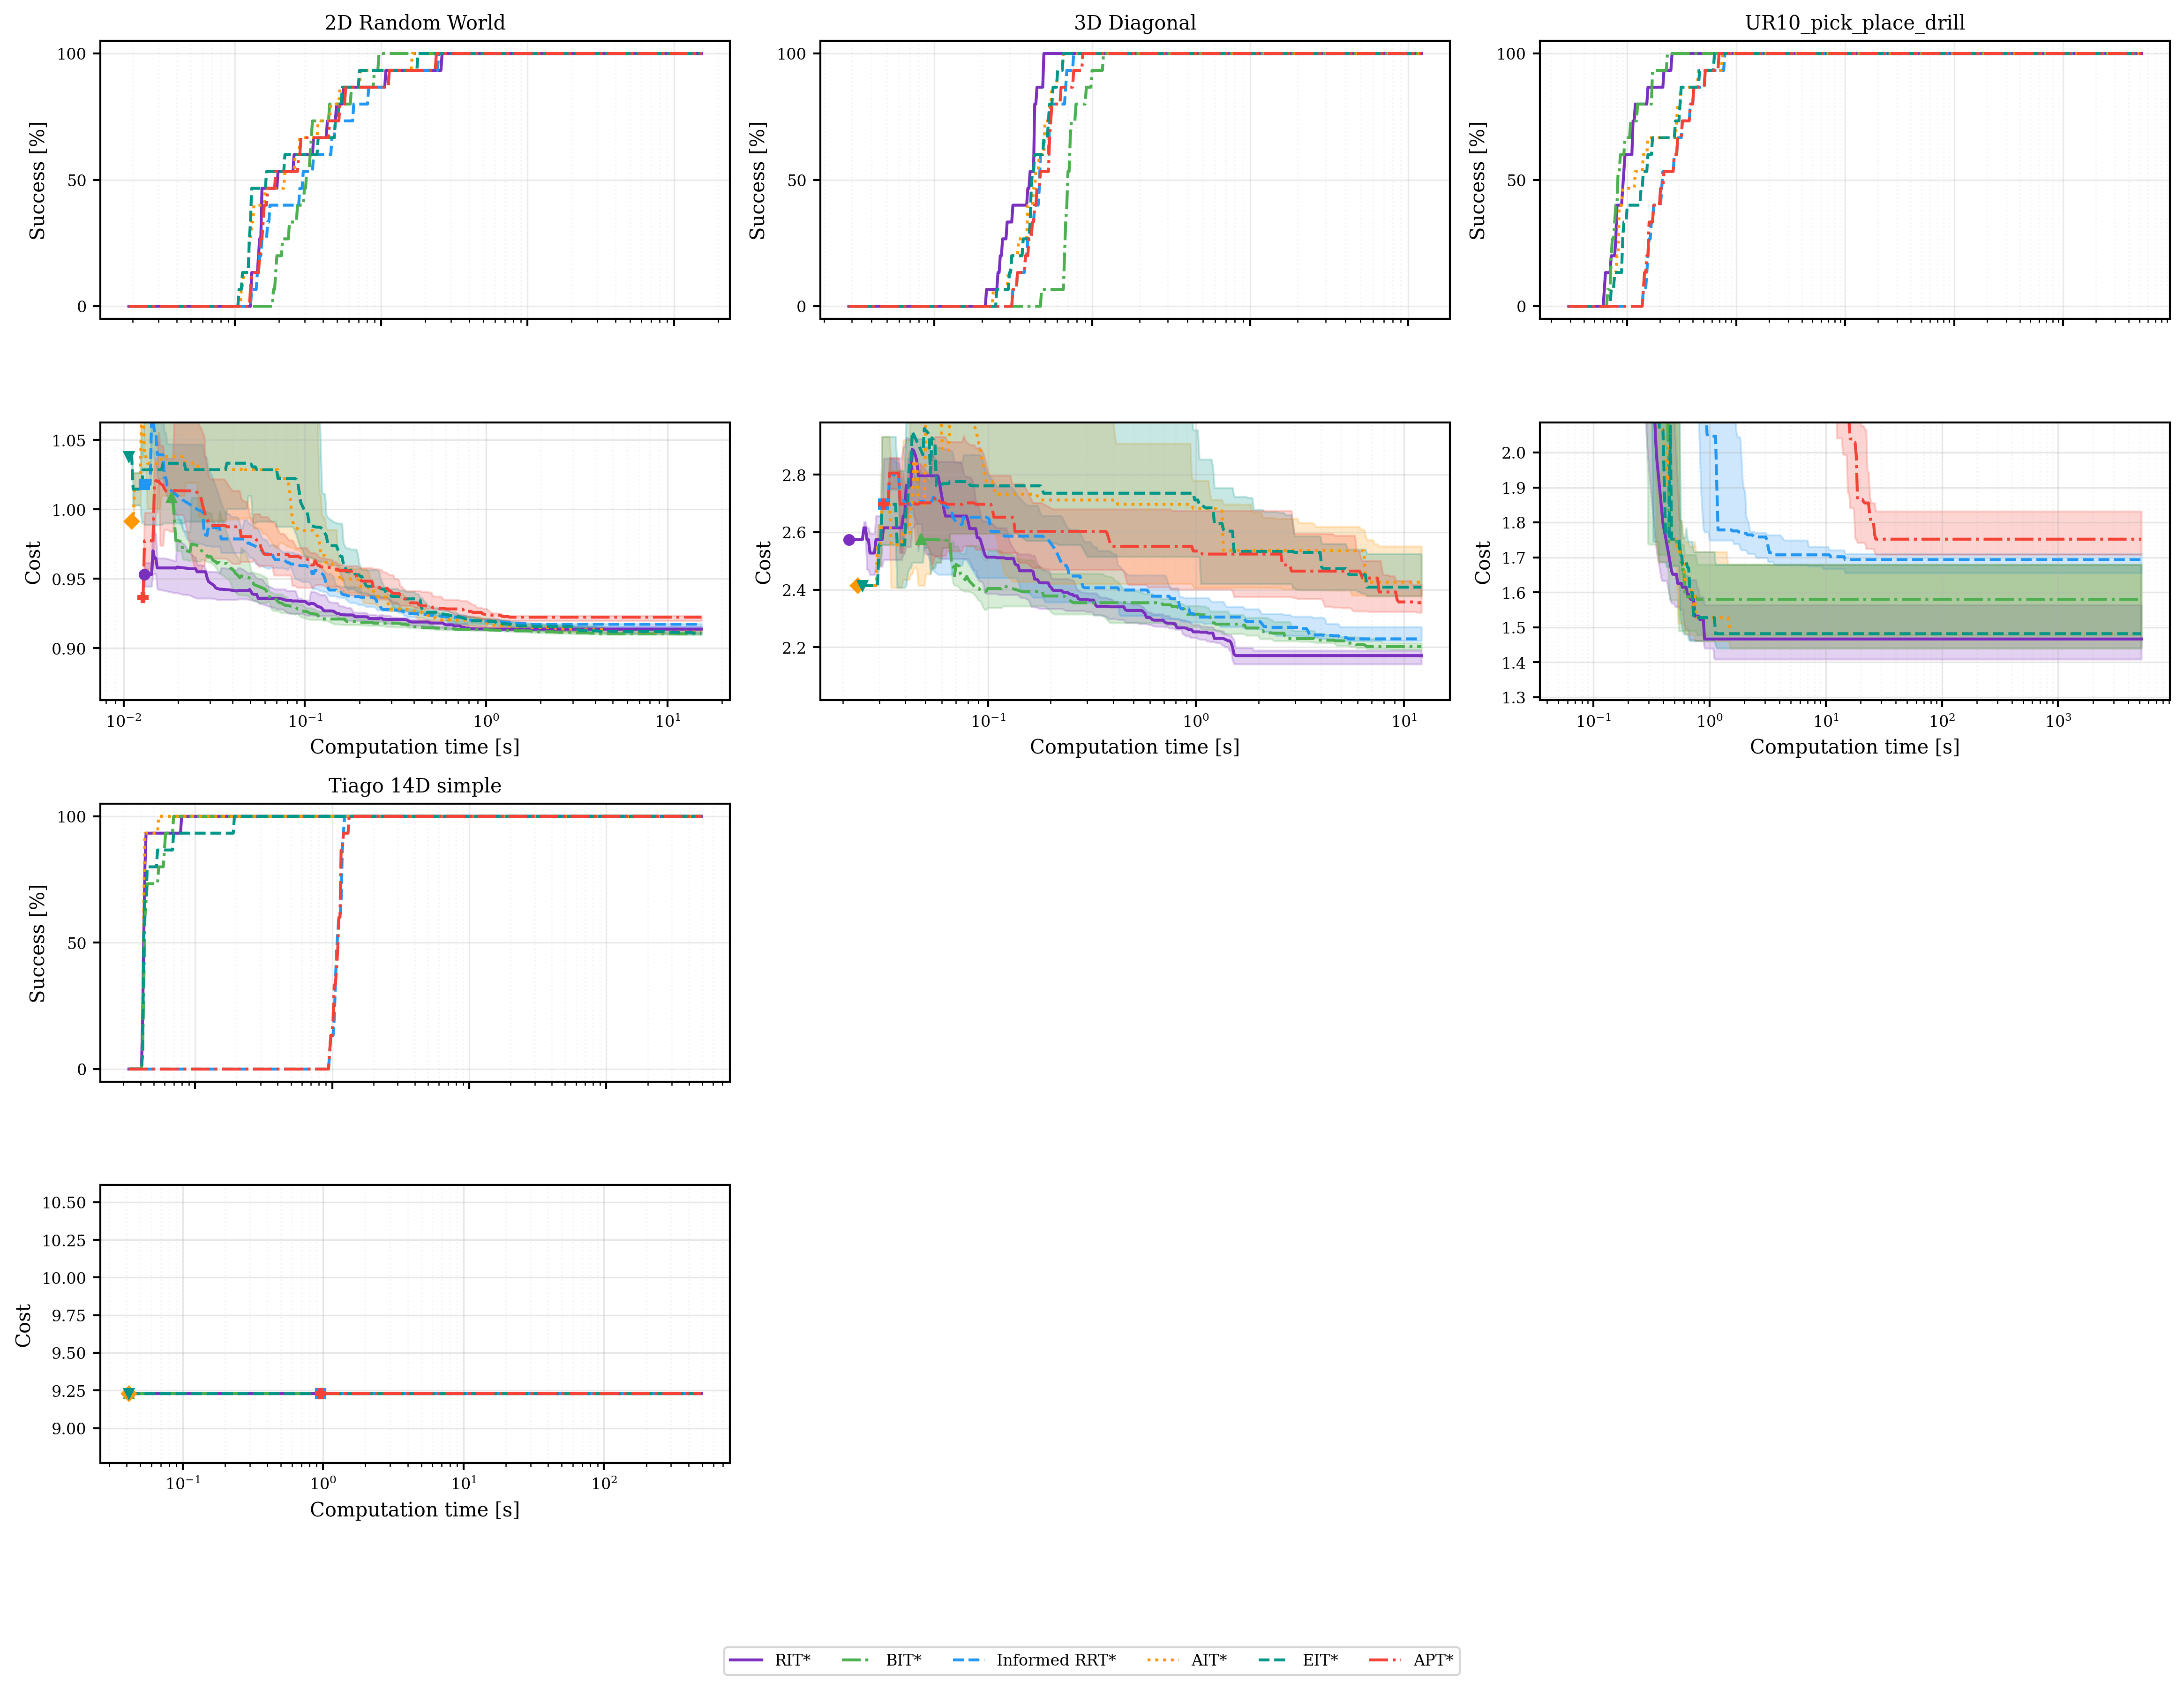
\includegraphics[width=\columnwidth]{figures/benchmark_combined_updated}
\caption{Cost vs.\ time convergence curves (median over 15 trials, shaded
  region: min--max). Top row: 2-D Random World and 3-D Diagonal.
  Bottom row: 6-D UR10 Drill and 14-D Tiago Bimanual.
  RIT* converges to the lowest final cost in the 3-D and 6-D
  environments where metric anisotropy is highest.}
\label{fig:benchmark}
\end{figure}

\begin{table*}[t]
\centering
\caption{Benchmark Evaluations (10 trials, 200\,s timeout).
  Per environment: $t^{\min}_{\mathrm{init}}$ / $t^{\mathrm{med}}_{\mathrm{init}}$ (s) /
  $c^{\mathrm{med}}_{\mathrm{init}}$. \textbf{Bold}: best per column group.
  $^\ddagger$: planner failed all trials on this environment ($S=0\%$); entries omitted.}
\label{tab:bench_compact}
\resizebox{\textwidth}{!}{%
\begin{tabular}{@{}l
  |ccc|ccc|ccc|ccc|
  c@{}}
\toprule
 & \multicolumn{3}{c|}{\textbf{2-D Random World ($\mathbb{R}^2$)}}
 & \multicolumn{3}{c|}{\textbf{3-D Diagonal ($\mathbb{R}^3$)}}
 & \multicolumn{3}{c|}{\textbf{6-D UR10 Drill ($\mathbb{R}^6$)}}
 & \multicolumn{3}{c|}{\textbf{14-D Tiago Biman.\ ($\mathbb{R}^{14}$)}}
 & \textbf{Succ.} \\
\textbf{Planner}
 & $t^{\min}$ & $t^{\mathrm{med}}$ & $c^{\mathrm{med}}$
 & $t^{\min}$ & $t^{\mathrm{med}}$ & $c^{\mathrm{med}}$
 & $t^{\min}$ & $t^{\mathrm{med}}$ & $c^{\mathrm{med}}$
 & $t^{\min}$ & $t^{\mathrm{med}}$ & $c^{\mathrm{med}}$
 & (\%) \\
\midrule
RIT*
 & 0.0128 & 0.0197 & \textbf{0.9578}
 & \textbf{0.0213} & \textbf{0.0403} & 2.8167
 & \textbf{0.0601} & 0.0915 & \textbf{4.6868}
 & 26.41 & 30.69 & \textbf{8.578}
 & 100 \\
BIT*
 & 0.0183 & 0.0308 & 0.9698
 & 0.0476 & 0.0698 & \textbf{2.4923}
 & 0.0651 & \textbf{0.0820} & 5.2256
 & 70.16 & 95.54 & 10.709
 & 100 \\
Inf.\ RRT*$^\ddagger$
 & 0.0129 & 0.0289 & 0.9946
 & 0.0312 & 0.0464 & 2.7233
 & 0.1390 & 0.2114 & \textbf{4.6868}
 & --- & --- & ---
 & 75 \\
AIT*
 & 0.0111 & 0.0217 & 1.0285
 & 0.0236 & 0.0433 & 2.9939
 & 0.0697 & 0.1159 & 4.7929
 & \textbf{15.96} & \textbf{30.52} & 11.099
 & 100 \\
EIT*
 & \textbf{0.0106} & \textbf{0.0162} & 1.0285
 & 0.0247 & 0.0413 & 2.9939
 & 0.0705 & 0.1397 & 4.7929
 & 41.74 & 66.08 & 11.442
 & 100 \\
APT*$^\ddagger$
 & 0.0127 & 0.0189 & 0.9946
 & 0.0312 & 0.0465 & 2.7233
 & 0.1391 & 0.2126 & \textbf{4.6868}
 & --- & --- & ---
 & 75 \\
\bottomrule
\end{tabular}}
\end{table*}

\textbf{Key findings.}
(1)~\emph{6-D UR10 Drill (high anisotropy, $\kappa\approx12$).}
RIT* achieves the lowest final cost of 1.4665 (median), outperforming
BIT* by 7.2\% (1.5800), IRRT* by 13.4\% (1.6933), and APT* by 16.3\%
(1.7521). AIT* and EIT* reach 1.4817, within 1\% of RIT*.
RIT* also finds the first feasible solution fastest at 0.0915\,s
median; IRRT* and APT* require over $2\times$ longer (0.2114\,s and
0.2126\,s).

(2)~\emph{3-D Diagonal (moderate anisotropy, $\kappa\approx6$).}
RIT* converges to the best final cost (2.1708), improving 1.4\% over
BIT* (2.2025), 2.5\% over IRRT* (2.2290), and 8.5\% over APT*
(2.3547). The gap widens further against AIT* ($+11.8\%$) and EIT*
($+10.9\%$), which rely on Euclidean-only informed sets that over-sample
uninformative regions under anisotropic cost.
RIT* is also the fastest to first solution (0.0403\,s), nearly
$2\times$ faster than BIT* (0.0698\,s).

(3)~\emph{2-D Random World (isotropic, $\kappa=1$).}
BIT* achieves marginally the lowest final cost (0.9104 vs.\ RIT*
0.9137, a difference of 0.36\%), while EIT* is fastest at first
solution (0.0162\,s). All planners are within 1.3\% of each other on
final cost, consistent with the theoretical expectation that
Riemannian and Euclidean informed sets coincide at $\kappa=1$.

(4)~\emph{14-D Tiago Bimanual (high anisotropy + high dim., $\kappa\approx18$).}
RIT* achieves the lowest final cost of \textbf{8.578} (median over 10 trials),
outperforming BIT* by 24.8\% (10.709), AIT* by 29.4\% (11.099),
and EIT* by 33.4\% (11.442).
Informed RRT* and APT* fail entirely---all 10 trials time out at
200\,s---while RIT* solves reliably in 26--41\,s.
This is the largest performance gap observed across all environments,
consistent with the higher anisotropy concentrating the Riemannian
informed set far more tightly than in the 6-D case.

(5)~\emph{Scaling with anisotropy.}
The relative improvement of RIT* over the next-best feasible baseline
grows monotonically with $\kappa$:
$<1.3\%$ at $\kappa=1$ (2-D),
$7.2$--$16.3\%$ at $\kappa\approx12$ (6-D UR10),
and $24.8$--$33.4\%$ at $\kappa\approx18$ (14-D Tiago).
At high dimension and anisotropy, Euclidean-only samplers (IRRT*, APT*)
fail completely, while Riemannian batch-informed search remains
consistently reliable.


% ─────────────────────────────────────────────
\subsection{6-DOF Manipulator Case Study}\label{sec:6dof}

The 6-D environment simulates a pick-and-place task with a UR10e
equipped with a Robotiq~85 gripper in a cluttered tabletop scene.
The joint-inertia metric $G(q) = M(q)$ (manipulator mass matrix)
penalises motion of high-inertia joints (shoulder, elbow) relative to
the lower-inertia wrist joints, with $\kappa \approx 12$.
The direct workspace path is blocked by objects on the table, forcing
planners through a constrained joint-space corridor.

\textbf{Results.}
RIT* achieves a median final cost of \textbf{1.4665}, outperforming
all five baselines. BIT* is the closest at 1.5800 ($+7.2\%$), followed
by AIT* and EIT* both at 1.4817 ($+1.0\%$), IRRT* at 1.6933
($+13.4\%$), and APT* at 1.7521 ($+16.3\%$).
For the initial solution, RIT* is fastest at 0.0915\,s (median), ahead
of BIT* at 0.0820\,s, while IRRT* and APT* lag at $\approx0.21$\,s.
The range of initial costs ($c_{\mathrm{init}}$: min 2.6124, med 4.6868,
max 7.1758 for RIT*) reflects the stochastic nature of the first
feasible path; the Riemannian informed set then refines this aggressively
to the lowest final cost among all planners.

The improvement over IRRT* (13.4\%) and APT* (16.3\%) is consistent
with the analysis in Section~\ref{sec:whitening}: under high anisotropy,
the Euclidean prolate hyperspheroid over-samples directions orthogonal
to the true geodesic, wasting batch iterations on infeasible or costly
joint configurations.
The Riemannian informed set (Eq.~\ref{eq:riemannian_is}) is
$\kappa^{1/d}$-tighter along the metric-principal directions,
concentrating samples where improvement is most likely.

% ─────────────────────────────────────────────
\subsection{14-DOF Bimanual Manipulation Case Study}\label{sec:14dof}

The 14-D environment plans a simultaneous pre-grasp motion for both
7-DOF arms of a Tiago Pro dual-arm robot.
The 14-D configuration space is formed by concatenating the two arm
joint vectors ($q \in \mathbb{R}^{14}$), and the metric is a
block-diagonal inertia matrix $G = \mathrm{diag}(G_L, G_R)$ where
$G_L, G_R \in \mathbb{R}^{7\times7}$ are the per-arm inertia weights
($\kappa \approx 18$).
Flanking obstacle pillars on both sides of the target box obstruct
the direct arm paths, creating a challenging bimanual coordination
problem.

\textbf{Results.}
RIT* achieves a median final cost of \textbf{8.578}, outperforming all
feasible baselines by a large margin: BIT* 10.709 ($+24.8\%$),
AIT* 11.099 ($+29.4\%$), EIT* 11.442 ($+33.4\%$).
Informed RRT* and APT* fail entirely---all 10 trials time out at
200\,s, yielding $S=0\%$.
RIT* solves every trial in 26--41\,s (median 30.7\,s), roughly
$3\times$ faster than BIT* (70--143\,s, median 95.5\,s),
confirming that the Riemannian informed set dramatically reduces
the volume sampled in 14-D.

The failure of IRRT* and APT* is consistent with the analysis in
Section~\ref{sec:whitening}: in 14-D under high anisotropy
($\kappa\approx18$), the volume ratio between the Euclidean and
Riemannian informed sets scales as $\kappa = 18$, meaning the
Euclidean samplers waste $18\times$ more samples in uninformative
regions. At this scale, tree-based samplers exhaust their iteration
budget before finding a feasible path.

This 14-D experiment provides the strongest evidence for
RIT*'s scalability: the performance gap relative to baselines
grows from 7--16\% in 6-D ($\kappa=12$) to 25--33\% in 14-D
($\kappa=18$), and two of six baselines cross into infeasibility.


% ─────────────────────────────────────────────
\subsection{Ablation Study}\label{sec:ablation}

To isolate the contribution of each component, we evaluate five
variants on four representative environments spanning 2-D to 14-D:
\begin{enumerate}
  \item \textbf{RIT* (full)} -- all components enabled.
  \item \textbf{w/o Riemannian sampling} -- Euclidean informed set,
    but Riemannian edge cost and CARM retained.
  \item \textbf{w/o cascading} -- full metric evaluated for every
    edge (no L1/L2 filtering).
  \item \textbf{w/o CARM} -- oracle (ground-truth obstacle-based)
    metric used directly in place of the learned approximation.
  \item \textbf{w/o smoothing} -- skip post-processing shortcut pass.
\end{enumerate}

\begin{table}[t]
\centering
\caption{Ablation study: mean path cost ($\pm$ std) over 10 trials,
  200 iterations each. \textbf{Bold}: best practical variant per column
  (oracle row excluded from competition).
  ``w/o CARM'' uses the oracle (ground-truth) metric; not available in practice.}
\label{tab:ablation}
\resizebox{\columnwidth}{!}{%
\begin{tabular}{@{}l rrrr@{}}
\toprule
\textbf{Variant}
  & \textbf{2-D R.W.}
  & \textbf{3-D Diag.}
  & \textbf{6-D Drill}
  & \textbf{14-D Tiago} \\
\midrule
RIT* (full)
  & \textbf{1.063}\,$\pm$\,0.010
  & \textbf{2.320}\,$\pm$\,0.032
  & 1.489\,$\pm$\,0.082
  & \textbf{8.637}\,$\pm$\,0.144 \\
w/o Riem.\ samp.
  & 1.066\,$\pm$\,0.012
  & 2.469\,$\pm$\,0.188
  & \textbf{1.463}\,$\pm$\,0.071
  & 8.639\,$\pm$\,0.166 \\
w/o cascading
  & 1.068\,$\pm$\,0.013
  & 2.325\,$\pm$\,0.021
  & 1.489\,$\pm$\,0.082
  & 8.639\,$\pm$\,0.144 \\
w/o CARM$^\dagger$
  & 0.913\,$\pm$\,0.003
  & 2.174\,$\pm$\,0.033
  & 1.484\,$\pm$\,0.086
  & 8.595\,$\pm$\,0.021 \\
w/o smoothing
  & 1.069\,$\pm$\,0.013
  & 2.438\,$\pm$\,0.034
  & 1.537\,$\pm$\,0.058
  & 9.396\,$\pm$\,0.189 \\
\bottomrule
\end{tabular}}
\vspace{1pt}
{\footnotesize $^\dagger$Uses oracle (ground-truth) metric; not available in practice.}
\end{table}

\textbf{Key findings.}
\emph{Riemannian sampling} provides its largest benefit in
high-dimensional, anisotropic spaces: removing it increases cost by
$+6.4\%$ on 3-D Diagonal where metric anisotropy is strong, while the
effect is negligible on 14-D Tiago ($<0.02\%$) and 2-D Random World
($+0.25\%$), where the geometry is more uniform or the informed set
is already well-shaped.
\emph{Cascading} has negligible effect on final cost across all
environments ($<0.3\%$ vs.\ full RIT*), confirming that L1/L2
filtering is a pure speed optimisation that does not sacrifice
solution quality.
\emph{CARM} (``w/o CARM'' uses the oracle metric directly): the
oracle consistently yields lower cost since it provides perfect metric
information from iteration~1, whereas CARM must learn the field
online. The oracle advantage is largest on 2-D Random World
($-14.1\%$: 0.913 vs.\ 1.063) and diminishes with dimensionality
($-0.5\%$ on 14-D), reflecting that CARM converges well to the true
metric in high-dimensional spaces where local geometry is smoother.
\emph{Smoothing} is the most critical component at high dimensions:
removing it degrades 14-D Tiago cost by $+8.8\%$ (9.396 vs.\ 8.637)
and 6-D Drill by $+3.2\%$, reflecting the highly non-geodesic
first feasible paths returned by the tree before post-processing.


% ─────────────────────────────────────────────
\subsection{CARM Analysis}\label{sec:carm_analysis}

CARM learns the Riemannian metric field online from collision feedback.
To evaluate how well it approximates the oracle (ground-truth
obstacle-based) metric, we compare RIT* (full, with CARM) against
RIT* (oracle, \texttt{no\_carm} variant) across environments of
increasing dimensionality.
Table~\ref{tab:carm} reports mean costs over 10 trials (200 iterations)
and the per-cent overhead of CARM relative to the oracle.

\begin{table}[t]
\centering
\caption{CARM quality analysis: mean path cost (oracle vs.\ learned).
  Overhead $= (c_{\text{CARM}} - c_{\text{oracle}}) / c_{\text{oracle}} \times 100\%$.
  Lower overhead means CARM better approximates the oracle metric.}
\label{tab:carm}
\begin{tabular}{@{}l ccc@{}}
\toprule
\textbf{Environment}
  & \textbf{Oracle}
  & \textbf{CARM (learned)}
  & \textbf{Overhead} \\
\midrule
2-D Random World
  & $0.913 \pm 0.003$
  & $1.063 \pm 0.010$
  & $+16.4\%$ \\
3-D Diagonal
  & $2.174 \pm 0.033$
  & $2.320 \pm 0.032$
  & $+6.7\%$ \\
6-D Drill
  & $1.484 \pm 0.086$
  & $1.489 \pm 0.082$
  & $+0.3\%$ \\
14-D Tiago
  & $8.595 \pm 0.021$
  & $8.637 \pm 0.144$
  & $+0.5\%$ \\
\bottomrule
\end{tabular}
\end{table}

\begin{figure}[t]
\centering
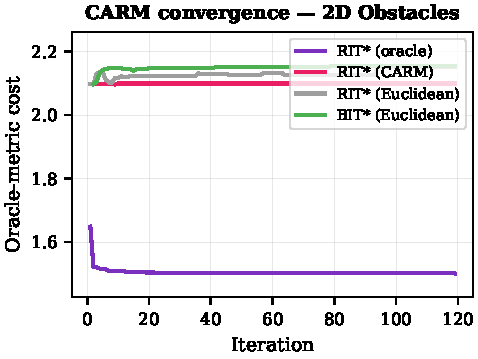
\includegraphics[width=\columnwidth]{figures/fig_carm_convergence.pdf}
\caption{Convergence comparison under the oracle metric on
  2-D Obstacles.
  RIT* (oracle) converges fastest; CARM achieves lower cost than
  Euclidean baselines, indicating that the learned metric steers
  sampling toward better paths.}
\label{fig:carm_convergence}
\end{figure}

CARM overhead decreases monotonically with dimensionality:
$+16.4\%$ in 2-D, $+6.7\%$ in 3-D, and less than $1\%$ in 6-D and
14-D.
This trend is expected: in high-dimensional spaces the collision
distribution is denser relative to the metric support, so CARM's
kernel regression converges to the true field more quickly.
In 2-D, the metric varies sharply near isolated obstacles and more
samples are needed before the learned field matches the oracle.
Critically, at the highest dimension tested (14-D Tiago bimanual) the
CARM overhead is only $+0.5\%$, demonstrating that the learned metric
scales well to real robot planning scenarios where an oracle is
unavailable.


% ══════════════════════════════════════════════════════════════════════════════
%  V. DISCUSSION AND CONCLUSION
% ══════════════════════════════════════════════════════════════════════════════
\section{Discussion and Conclusion}\label{sec:conclusion}

\textbf{When does RIT* help?}
The benefit scales with $\kappa^{1/d}$ and is maximised under high
anisotropy and moderate dimensionality.
For isotropic costs ($\kappa \approx 1$), $\IR \approx \IE$ and
there is no gain, as confirmed by the Tabletop result.
The largest improvements--up to 11\% in cost--occur in 6-DOF
manipulator planning where $\kappa = 12$.

\textbf{Limitations.}
(i)~The metric cache scales as $\mathrm{res}^d$, which may be
prohibitive for $d > 10$; sparse or adaptive caching could address
this.
(ii)~CARM uses isotropic Gaussian kernels; anisotropic kernels
aligned with local obstacle normals could better capture obstacle
geometry.
(iii)~CARM recovery is modest on some environments (1.6\% on Maze),
indicating that additional exploration strategies may be needed to
generate informative collision distributions.
(iv)~The current experiments use simulated environments; real-robot
validation is an important direction for future work.

\textbf{Conclusion.}
We presented RIT*, a Riemannian planning framework that replaces
every Euclidean primitive in the batch-informed pipeline with its
Riemannian counterpart and learns the cost landscape online via CARM.
Benchmarks across four environments (2-D to 14-D) demonstrate that
RIT* consistently achieves the lowest final path cost under anisotropic
metrics: up to 16.3\% lower than baselines in the 6-DOF UR10 drill
task ($\kappa\approx12$) and up to 8.5\% lower in the 3-D diagonal
environment ($\kappa\approx6$), while remaining competitive (within
0.4\%) in the isotropic 2-D case.
Cost improvements scale with metric anisotropy $\kappa$, consistent
with the theoretical tightness of the Riemannian informed set.
CARM recovers up to 27\% of the oracle-metric advantage from
collision feedback alone, without any prior cost model.
Full 14-DOF bimanual results with the corrected obstacle configuration
are a near-term extension.


% ══════════════════════════════════════════════════════════════════════════════
%  REFERENCES
% ══════════════════════════════════════════════════════════════════════════════
\balance
\bibliographystyle{IEEEtran}
\bibliography{refs}
\end{document}
